\documentclass{article}
\usepackage{tikz}
\usetikzlibrary{automata, positioning, arrows}

\begin{document}

\section*{CTL Model Checking}

Gegeben seien die atomaren Propositionen \( p \) und \( q \) und die Struktur 
\( K = (\{v1, v2, v3\}, \{(v1, v2), (v1, v3), (v2, v2)\}, L, \{v1\}) \), 
wobei \( L(v1) = \emptyset \), \( L(v2) = \{p\} \) und \( L(v3) = \{q\} \). 
Benutzen Sie den Algorithmus aus der Vorlesung, um \( K \models AF(p \land AX \neg q) \) zu entscheiden.

\begin{center}
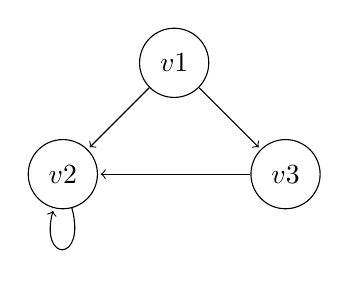
\begin{tikzpicture}[shorten >=1pt,node distance=2cm,on grid,auto] 
   \node[state] (v1) {\(v1\)};
   \node[state] (v2) [below left=of v1] {\(v2\)};
   \node[state] (v3) [below right=of v1] {\(v3\)};
    \path[->] 
    (v1) edge node {} (v2)
    (v1) edge node {} (v3)
    (v3) edge node {} (v2)
    (v2) edge [loop below] node {} ();
\end{tikzpicture}
\end{center}

\end{document}